\graphicspath{{images/}}
\section*{LGS und Matrizen}

\subsubsection*{Matrizen}

    \begin{definition}{{Matrix, Element, Zeilen, Spalten und Typ}}\\
        Eine \textit{Matrix} ist (simpel gesagt) ein Vektor mit mehreren Spalten 
        und wird mit Grossbuchstaben bezeichnet.
        Ein \textit{Element} $a_ij$ ist ein Wert aus dieser Matrix,
        auf den über die Zeile und Spalte zugegriffen wird (\textbf{Z}eile \textbf{z}uerst,
        \textbf{Sp}alte \textbf{Sp}äter).
        Der \textit einer Matrix ergibt sich aus der Anzahl ihren Zeilen und Spalten.
        Matrizen mit $m$-Zeilen und $n$-Spalten werden $m\times n$-Matrizen genannt.
    \end{definition}

    \begin{concept}{Matrix}
        Tabelle mit $m$ Zeilen und $n$ Spalten.
        \begin{itemize}
            \item $m \times n$-Matrix
            \item $a_{ij}$: Element in der $i$-ten Zeile und $j$-ten Spalte
        \end{itemize}
    \end{concept}

    \begin{definition}{Nullmatrix}
        Eine Matrix, deren Elemente alle gleich $0$ sind, heisst \textit{Nullmatrix} und wird mit $0$ bezeichnet.
    \end{definition}

    \begin{definition}{Spaltenmatrix}
        Besteht eine Matrix nur aus einer Spalte, so heisst diese \textit{Spaltenmatrix}.
        Können als Vektoren aufgefasst werden und können mit einem kleinen Buchstaben 
        sowie einem Pfeil darüber notiert werden ($\vec{a}$). 
    \end{definition}
    
    \begin{minipage}{0.5\linewidth}
    \begin{formula}{Addition und Subtraktion}
        \begin{itemize}
            \item $A + B = C$
            \item $c_{ij} = a_{ij} + b_{ij}$
        \end{itemize}
    \end{formula}
    \end{minipage}
    \begin{minipage}{0.5\linewidth}
    \begin{formula}{Skalarmultiplikation}
        \begin{itemize}
            \item $k \cdot A = B$
            \item $b_{ij} = k \cdot a_{ij}$
        \end{itemize}
    \end{formula}
    \end{minipage}

    \begin{theorem}{Rechenregeln für die Addition und skalare Multiplikation von Matrizen}
        \begin{itemize}
            \item Kommutativ-Gesetz: $A+B=B+A$
            \item Assoziativ-Gesetz: $A+(B+C)=(A+B)+C$
            \item Distributiv-Gesetz:\\ 
                $\lambda\cdot(A+B)=\lambda\cdot A+\lambda\cdot B$
                sowie $(\lambda + \mu)\cdot A=\lambda\cdot A+\mu\cdot A$
        \end{itemize}    
    \end{theorem}
    
    \begin{formula}{Matrixmultiplikation} $A^{m \times n}$, $B^{n \times k}$\\
        \begin{minipage}{0.6\linewidth}
        Bedingung: $A$ $n$ Spalten, $B$ $n$ Zeilen.\\
        Resultat: $C$ hat $m$ Zeilen und $k$ Spalten.
        \begin{itemize}
            \item $A \cdot B = C$
            \item $c_{ij} = a_{i1} \cdot b_{1j} + a_{i2} \cdot b_{2j} + \ldots + a_{in} \cdot b_{nj}$
            \item $A \cdot B \neq B \cdot A$
        \end{itemize}  
        \end{minipage}
        \begin{minipage}{0.35\linewidth} 
        \begin{center}
        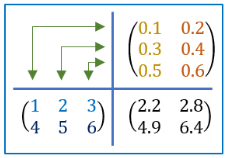
\includegraphics[width=0.8\linewidth]{images/matrixmultiplikation.png}
        \end{center}
        \end{minipage}
    \end{formula}


    
    
    \begin{theorem}{Rechenregeln für die Multiplikation von Matrizen}
        \begin{itemize}
            \item Assoziativ-Gesetz: $A\cdot(B\cdot C)=(A\cdot B)\cdot C$
            \item Distributiv-Gesetz: \\
                $A\cdot(B+C)=A\cdot B+A\cdot C$ und $(A+B)\cdot C=A\cdot C+B\cdot C$
            \item Skalar-Koeffizient: $(\lambda\cdot A)\cdot B=\lambda\cdot (A\cdot B)=A\cdot(\lambda\cdot B)$
        \end{itemize}
    \end{theorem}

    \begin{minipage}{0.65\linewidth}
        \begin{definition}{Transponierte Matrix} $A^{m \times n} \rightarrow (A^T)^{n \times m}$
            \begin{itemize}
                \item $A^T$: Spalten und Zeilen vertauscht
                \item $(A^T)_{ij} = A_{ji}$
            \end{itemize}
            \vspace{2mm}
            $${(A\cdot B)}^T = B^T\cdot A^T$$
        \end{definition}
    \end{minipage}
    \begin{minipage}{0.35\linewidth}
        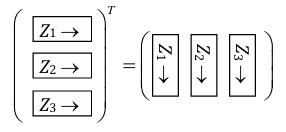
\includegraphics[width=1\linewidth]{images/mat-transpos.png}
    \end{minipage}

    \begin{KR}{Spezielle Matrizen}
        \begin{itemize}
            \item \textbf{Symmetrische Matrix}: $A^T = A$
            \item \textbf{Einheitsmatrix}: $E$ mit $e_{ij} = 1$ für $i = j$ und $e_{ij} = 0$ für $i \neq j$
            \item \textbf{Diagonalmatrix}: $a_{ij} = 0$ für $i \neq j$
            \item \textbf{Dreiecksmatrix}: $a_{ij} = 0$ für $i > j$ (obere Dreiecksmatrix) \\oder $i < j$ (untere Dreiecksmatrix)
        \end{itemize}
    \end{KR}

\raggedcolumns
\columnbreak

\subsubsection*{Lineare Gleichungssysteme (LGS)}
    
        \begin{definition}{Lineares Gleichungssystem (LGS)}
            Ein \textit{lineares Gleichungssystem} ist eine Sammlung von Gleichungen, 
            die linear in den Unbekannten sind. 
            Ein LGS kann in Matrixform $A\cdot\vec{x}=\vec{b}$ dargestellt werden.\\
            \begin{minipage}
                {0.45\linewidth}
                {\small
                $A$: Koeffizientenmatrix\\
                $\vec{x}$: Vektor der Unbekannten\\
                $\vec{b}$: Vektor der Konstanten}
            \end{minipage}
            \begin{minipage}{0.55\linewidth}
                $\begin{psmallmatrix} a_{11} & \cdots & a_{1n} \\ \scalebox{0.5}{\vdots} & \cdots & \scalebox{0.5}{\vdots} \\ a_{m1} & \cdots & a_{mn} \end{psmallmatrix} \cdot \begin{psmallmatrix}
                    x_1 \\ \scalebox{0.5}{\vdots} \\ x_n
                \end{psmallmatrix} = \begin{psmallmatrix}
                    b_1 \\ \scalebox{0.5}{\vdots} \\ b_m
                \end{psmallmatrix}$
            \end{minipage}
        \end{definition}

    
        \begin{theorem}{Rang einer Matrix} $rg(A)$ = Anzahl Zeilen - Anzahl Nullzeilen
            
            $\Rightarrow$ Anzahl linear unabhängiger Zeilen- oder Spaltenvektoren
        \end{theorem}


\begin{concept}{Zeilenstufenform (Gauss)}
    \begin{itemize}
        \item Alle Nullen stehen unterhalb der Diagonalen, Nullzeilen zuunterst
        \item Die erste Zahl $\neq 0$ in jeder Zeile ist eine führende Eins
        \item Führende Einsen, die weiter unten stehen $\rightarrow$ stehen weiter rechts
    \end{itemize}
    \textbf{Reduzierte Zeilenstufenform: (Gauss-Jordan)}\\
    Alle Zahlen links und rechts der führenden Einsen sind Nullen.
\end{concept}
    
    \begin{formula}{Gauss-Jordan-Verfahren}
        \begin{enumerate}
            \item bestimme linkeste Spalte mit Elementen $\neq 0$ (Pivot-Spalte)
            \item oberste Zahl in Pivot-Spalte $= 0$\\ $\rightarrow$ vertausche Zeilen so dass $a_{11} \neq 0$
            \item teile erste Zeile durch $a_{11}$ $\rightarrow$ so erhalten wir führende Eins
            \item Nullen unterhalb führender Eins erzeugen (Zeilenperationen)
        \end{enumerate}
        nächste Schritte: ohne bereits bearbeitete Zeilen Schritte 1-4 wiederholen, bis Matrix Zeilenstufenform hat
    \end{formula}

    \begin{KR}{Zeilenperationen} erlaubt bei LGS (z.B. Gauss-Verfahren)
        \begin{itemize}
            \item Vertauschen von Zeilen
            \item Multiplikation einer Zeile mit einem Skalar
            \item Addition eines Vielfachen einer Zeile zu einer anderen
        \end{itemize}
    \end{KR}

    \begin{theorem}{Lösbarkeit von linearen Gleichungssystemen}

        \begin{minipage}{0.5\linewidth}
            \begin{itemize}
                \item Lösbar: $rg(A) = rg(A|b)$
                \item genau eine Lösung: $rg(A) = n$
            \end{itemize}
        \end{minipage}
        \begin{minipage}{0.5\linewidth}
            \begin{itemize}
                \item unendlich viele Lösungen:\\ $rg(A) < n$
            \end{itemize}
        \end{minipage}
    \end{theorem}

    \begin{KR}{Parameterdarstellung} bei unendlich vielen Lösungen

        \begin{minipage}{0.74\linewidth}
            Führende Unbekannte: Spalte mit führender Eins\\
            Freie Unbekannte: Spalten ohne führende Eins
        \end{minipage}
        \begin{minipage}{0.25\linewidth}
            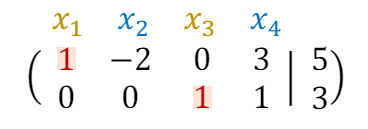
\includegraphics[width=1\linewidth]{images/parameterdarstellung_lgs.png}
        \end{minipage}

        \vspace{1mm}
        
        Auflösung nach der führenden Unbekannten:
        \begin{itemize}
            \item $1 x_1 - 2 x_2 + 0 x_3 + 3 x_4 = 5 \quad x_2 = \lambda \rightarrow x_1 = 5 + 2 \cdot \lambda - 3 \cdot \mu$
            \item $0 x_1 + 0 x_2 + 1 x_3 + 1 x_4 = 3 \quad x_4 = \mu \rightarrow x_3 = 3 - \mu$    
        \end{itemize}
        \vspace*{2mm}
        $$ \vec{x} = \begin{psmallmatrix} x_1 \\ x_2 \\ x_3 \\ x_4 \end{psmallmatrix} 
        = \begin{psmallmatrix} 5 + 2 \lambda - 3 \mu \\ \lambda \\ 3 - \mu \\ \mu \end{psmallmatrix} 
        = \begin{psmallmatrix} 5 \\ 0 \\ 3 \\ 0 \end{psmallmatrix} + \lambda \begin{psmallmatrix} 2 \\ 1 \\ 0 \\ 0 \end{psmallmatrix} + \mu \begin{psmallmatrix} -3 \\ 0 \\ -1 \\ 1 \end{psmallmatrix}$$
    \end{KR}

    \begin{definition}{Homogenes LGS}
        $\vec{b}=\vec{0} \rightarrow A\cdot\vec{x}=\vec{0} \rightarrow rg(A)=rg(A\mid\vec{b})$\\
        nur zwei Möglichkeiten:
            \begin{itemize}
                \item eine Lösung $x_1=x_2=\cdots=x_n=0$, die sog. \textit{triviale Lösung}.
                \item unendlich viele Lösungen
            \end{itemize}
    \end{definition}

    \begin{theorem}{Koeffizientenmatrix{,} Determinante{,} Lösbarkeit des LGS }\\
        Für $n\times n$-Matrix $A$ sind folgende Aussagen äquivalent:
    
        \vspace{1mm}
    
        \begin{minipage}{0.3\linewidth}
            \begin{itemize}
                \item $\det(A)\neq 0$
                \item $rg(A)=n$
                \item $A$ ist invertierbar
            \end{itemize}
        \end{minipage}
        \begin{minipage}{0.7\linewidth}
            \begin{itemize}
                \item Spalten von $A$ sind linear unabhängig.
                \item Zeilen von $A$ sind linear unabhängig.
                \item LGS $A\cdot\vec{x}=\vec{0}$ \\hat eindeutige Lösung $x=A^{-1}\cdot 0=0$
            \end{itemize}
        \end{minipage}
    \end{theorem}


  

\subsubsection*{Quadratische Matrizen}



\begin{formula}{Umformen}
    bestimme die Matrix $X$:
    $A \cdot X + B = 2 \cdot X$

    \vspace{1mm}

    $
    \Rightarrow A \cdot X = 2 \cdot X - B \Rightarrow A \cdot X - 2 \cdot X = -B \Rightarrow (A - 2 \cdot E) \cdot X = -B \\
    \Rightarrow (A - 2 \cdot E) \cdot (A - 2 \cdot E)^{-1} \cdot X = (A - 2 \cdot E)^{-1} \cdot -B \\
    \Rightarrow X = (A - 2 \cdot E)^{-1} \cdot -B
    $
\end{formula}

\paragraph{Inverse}
    \begin{definition}{Inverse einer quadratischen Matrix A} $A^{-1}$ 
        
        $A^{-1}$ existiert, wenn $rg(A) = n$. $A^{-1}$ ist eindeutig bestimmt.

        \vspace{1mm}

        {\small Eine Matrix heisst \textit{invertierbar / regulär}, wenn sie eine Inverse hat. 
        Andernfalls heisst sie \textit{singulär}}
    \end{definition}
  
    \begin{theorem}{Eigenschaften invertierbarer Matrizen}
        \begin{itemize}
            \item $A\cdot A^{-1}=A^{-1}\cdot A=E$
            \item $(A^{-1})^{-1}=A$
            \item ${(A\cdot B)}^{-1}=B^{-1}\cdot A^{-1}$ {\small $\quad$ Die Reihenfolge ist relevant!}\\ $A$ und $B$ invertierbar $\Rightarrow$ $AB$ invertierbar
            \item ${(A^T)^{-1}}={(A^{-1})}^T$ $\quad$ $A$ invertierbar $\Rightarrow$ $A^T$ invertierbar
        \end{itemize}
    \end{theorem}

\begin{theorem}{Inverse einer $2 \times 2$-Matrix} $A = \begin{psmallmatrix} a & b \\ c & d \end{psmallmatrix}$ mit $det(A) = ad - bc$
        $$A^{-1} = \frac{1}{\det(A)} \cdot \begin{pmatrix} d & -b \\ -c & a \end{pmatrix}$$
        NUR Invertierbar falls $ad - bc \neq 0$
\end{theorem}

\begin{KR}{Inverse berechnen} einer quadratischen Matrix $A^{n \times n}$
    $$A \cdot A^{-1} = E \rightarrow \left( A | E \right) \leadsto \text{Zeilenoperationen} \leadsto \left( E | A^{-1}\right)$$
\end{KR}

\begin{example}
    $$
\underbrace{\left(\begin{array}{ccc}
4 & -1 & 0 \\
0 & 2 & 1 \\
3 & -5 & -2
\end{array}\right)}_{A} \cdot \underbrace{\left(\begin{array}{lll}
x_{1} & y_{1} & z_{1} \\
x_{2} & y_{2} & z_{2} \\
x_{3} & y_{3} & z_{3}
\end{array}\right)}_{A^{-1}}=\underbrace{\left(\begin{array}{lll}
1 & 0 & 0 \\
0 & 1 & 0 \\
0 & 0 & 1
\end{array}\right)}_{E}$$
$$ \rightarrow\left(\begin{array}{ccc|ccc}
4 & -1 & 0 & 1 & 0 & 0 \\
0 & 2 & 1 & 0 & 1 & 0 \\
3 & -5 & -2 & 0 & 0 & 1
\end{array}\right)
$$

Zeilenstufenform (linke Seite)

$$ \leadsto 
\left(\begin{array}{ccc|ccc}
1 & -1 / 4 & 0 & 1 / 4 & 0 & 0 \\
0 & 1 & 1 / 2 & 0 & 1 / 2 & 0 \\
0 & 0 & 1 & -6 & 17 & 8
\end{array}\right)
$$

Reduzierte Zeilenstufenform (linke Seite)

$$ \leadsto 
\left(\begin{array}{ccc|ccc}
1 & 0 & 0 & 1 & -2 & -1 \\
0 & 1 & 0 & 3 & -8 & -4 \\
0 & 0 & 1 & -6 & 17 & 8
\end{array}\right) \Rightarrow A^{-1}=\left(\begin{array}{ccc}
1 & -2 & -1 \\
3 & -8 & -4 \\
-6 & 17 & 8
\end{array}\right)
$$
\end{example}



\begin{concept}{LGS mit Inverse lösen}
    $A \cdot \vec{x} = \vec{b}$
    $$A^{-1} \cdot A \cdot \vec{x} = A^{-1} \cdot \vec{b} \rightarrow \vec{x} = A^{-1} \cdot \vec{b}$$
    Beispiel:\\
    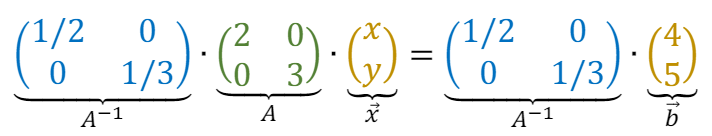
\includegraphics[width=0.7\linewidth]{images/lgs_inverse.png}
\end{concept}



